%
% Copyright (c) 2020 Antonio Coín Castro
%
% This work is licensed under a
% Creative Commons Attribution-ShareAlike 4.0 International License.
%
% You should have received a copy of the license along with this
% work. If not, see <http://creativecommons.org/licenses/by-sa/4.0/>.

In order to test our implementations, we will conduct a study to see how well our algorithms perform in a couple of real data sets. These data sets will of course present characteristics of Big Data, mainly the data volume. Before we begin, we would like to make some considerations.

\begin{enumerate}[1.]
  \item The main aspect of the algorithms we want to test, apart from their correctness, is their \textit{scalability}. This is not a study to designed to discern whether FRBS are better or worse than other classification or regression algorithms, though we will make comparisons with some of them for reference. That is to say, we do not intend to discuss the effectiveness of fuzzy systems, which has already been extensively established. What we do want to show is how the fuzzy algorithms we developed can function in an environment in which an arbitrary large amount of data is involved.
  \item Continuing along the lines of the previous point, we do not aim to get the best possible result with our algorithm either. That is why we will not be applying fine tuning techniques such as parameter grid search or cross validation. We will sometimes experiment with different configurations of parameters, but not in a systematic way.
  \item The data sets chosen for this study have a considerable number of instances, and present a challenge in the sense that a typical personal computer would struggle to process all the data into the algorithms. However, the limitations in the infrastructure available to test our implementations and the interest in making a sizeable number of executions with different parameters result in the choice of data sets with controlled size so that the execution time stays within reasonable margins.
\end{enumerate}

\section{Hardware and infrastructure}

We have deployed our programs on a dedicated server tailored for Big Data operations, called \verb|ulises.ugr.es|. This is a cluster of 20 machines interconnected and ready to execute Spark programs. The main characteristics of this architecture are as follows:

\begin{itemize}
  \item There are 20 nodes in total, each carrying 24 CPUs divided in 2 sockets, 6 cores per socket and 2 threads per core.
  \item Each individual CPU is an Intel(R) Xeon(R) CPU E5-2620 0 @ 2.00GHz.
  \item Each node has 64GB of memory.
  \item The Spark installation is currently at version 2.3.2. It uses YARN as the cluster manager and HDFS as the underlying distributed file system.
  \item The Scala version installed on this server is 2.11.8.
  \item The operating system is Ubuntu 18.04.2 LTS (GNU/Linux 4.15.0-74-generic x86\_64).
\end{itemize}

\section{Data sets}

We have selected five data sets in total for this experimentation. The first three of them are fit for classification problems (the data is labeled), and the last two are considered for regression purposes. We provide a very brief description of them below\footnote{All data sets used are publicly available at \url{https://archive.ics.uci.edu/ml/data sets.php}.}.

\begin{enumerate}[1.]
  \item \textit{HAR data set}. This is a ``small'' data set consisting on $165632$ instances of data gathered by sensors on the subject of human activity recognition. It possesses 18 numerical attributes (so we are working in $\R^{18}$) and 5 different class labels. For testing purposes, we make a 70\%-30\% train-test stratified split, resulting in the class distribution shown in Table \ref{tab:har-class}.

  \begin{table}[h!]
  \centering
  \caption{Class distribution for the HAR data set.}
  \label{tab:har-class}
  \begin{tabular}{cc}
    \toprule
Class & No. of instances \\ \midrule
  0              & 50631                \\
  1              & 11827                \\
  2              & 47370                \\
  3              & 12414                \\
  4              & 43390                \\
  \bottomrule
  \end{tabular}
  \end{table}
  \item \textit{POKER data set}. This data set is almost 10 times as big as the previous. It has 1025010 instances with 10 attributes and 10 classes, representing poker hands. The division in this case is 80\%-20\% for train and test, and the class distribution is imbalanced, but representative of the distribution we want to learn. The class distribution after the split can be seen in Table \ref{tab:poker-class}.

    \begin{table}[h!]
  \centering
  \caption{Class distribution for the POKER data set.}
  \label{tab:poker-class}
  \begin{tabular}{ccc}
    \toprule
Class & No. of training instances & No. of testing instances \\ \midrule
0              & 410960                                & 102741                       \\
1              & 346478                                & 86619                        \\
2              & 39062                                 & 9766                         \\
3              & 17308                                 & 4326                         \\
4              & 3182                                  & 796                          \\
5              & 1640                                  & 410                          \\
6              & 1168                                  & 292                          \\
7              & 189                                   & 47                           \\
8              & 13                                    & 4                            \\
9              & 7                                     & 1\\
  \bottomrule
  \end{tabular}
  \end{table}

\item \textit{SUSY data set}. This is a relatively large data set based on physics experiments, and is a well known reference for academic studies in Big Data (see \cite {baldi2014searching}). It has 5 million instances, 18 numerical attributes and 2 classes. We consider the first $4.5$ million points for training and the rest for testing. The class distribution is perfectly balanced in both cases.

\item \textit{Query Analytics Workloads data set (QAW)}. This is a regression synthetic data set, consisting of 199843 instances, 6 numerical attributes and one numerical variable to predict.

\item \textit{Gas Sensor Array data set (GSA)}. The last regression data set consists on a considerable higher number of instances, comparable to that of the SUSY data set. It consists of 4177504 instances with 16 numerical attributes and a numerical variable to predict. The data was gathered by a number of sensors measuring the concentration of some chemical compounds in a gas mixture under certain specific conditions.
\end{enumerate}

\section{Experimental results}

We proceed now with the results of the various scenarios considered. There are a couple of aspects that remain constant across all the executions, so we will briefly address them here. In the first place, we use the transformation \verb|StandardScaler| to standardize the data on each dimension and make it comparable, with mean $0$ and standard deviation $1$. Next, we fix the parameters in a call to Spark in order to use all the resources available, setting:

\begin{itemize}
  \item \verb|num-executors|: 20.
  \item \verb|executor-cores|: 19.
  \item \verb|executor-memory|: 32g.
\end{itemize}
We also fix the number of Spark partitions in 380 (1 partition per core) for every data set except SUSY and GSA, for which we consider 760 partitions (2 partitions per core). We tried to find a balance between the number of partitions and the size of the data set, since using many partitions when the number of points is not that big can lead to some unwanted situations. Moreover, we limit the number of iterations to 100 in iterative algorithms, and set the tolerance for stopping conditions at $\epsilon=10^{-4}$.

For the reasons explained in Chapter \ref{ch:implementation} we will only consider the implementation of the intermediate version of Chiu's algorithm, denoted ChiuI, for which we fix the number of groups to 10. In addition, when coupled with the FCM algorithm, we will always compare the results with the random initialization version using \textit{the number of centroids found with the subtractive clustering algorithm}.

The metric used to measure the quality of the algorithms will be the \textit{accuracy} in the case of classification problemas and the \textit{mean squared error} (\acrshort{mse}) in regression problems. In each case we will show the value of the metric on the test set and the execution time in minutes, denoted by $T$.

\subsection{Classification algorithms}

For comparison we have included some some well-known classification algorithms from the MLlib: a Random Forest classifier with 200 trees and Logistic Regression classifier with L2 regularization. We have also included the clustering algortihm K-Means, to which we have applied the same modification to turn it into a classification algorithm that we did with the Fuzzy C-Means algorithm. We present the results obtained on each of the first three data sets, showing the number of iterations, denoted by \#, and the cluster centers (if applicable). In addition, we will also show the value of the function being optimized in FCM. Firstly, the results of the HAR data set are available on Tables \ref{tab:har1}, \ref{tab:har2} and \ref{tab:har3}.

\begin{table}[h!]
  \centering
\caption{Experimental results of comparison algorithms for the HAR data set.}
\label{tab:har1}
\begin{tabular}{ccccc}
\toprule
Algorithm & Centroids & Acc& T & \# \\ \midrule
Random Forest & -- & \textbf{97.340} & 0.82 & -- \\
Logistic Regression & --& 83.411 & 0.53 & -- \\
\multirow{2}{*}{KMeans} & 150 & 93.001 & 1.08 & 59 \\
& 255 & 94.568 &  1.48 & 52\\
ChiuI & 255 & 70.892 &  1.03 & -- \\ \bottomrule
\end{tabular}
\end{table}

We observe that, as expected, the Random Forest classifier achieves a high accuracy and is the clear winner of this comparison. What is somewhat surprising is that the adapted KMeans algorithm beats the Logistic Regression model, which is specifically designed to perform well in multi-label classification problems. Both algorithms took roughly the same time to finish, and the KMeans model ended up 10 points ahead, which is quite a margin. Finally, the subtractive clustering algorithm performs worse than the rest, which was to be expected, since in general fuzzy algorithms trade a bit of accuracy for a better interpretability of the model. What is important to note here is that the fuzzy ChiuI algorithm appears to be scalable: it takes up about as much time as any of the other algorithms tried. We chose the value $r_a=1$ after some experimentation, and left the rest of the parameters with their default values.

\begin{table}[h!]
  \centering
\caption{Experimental results of the FCM algorithm with random initialization for the HAR data set.}
\label{tab:har2}
\begin{tabular}{ccccccccc}
\toprule
\multicolumn{3}{c}{Algorithm} & Centroids & Acc & Loss & T & \# \\ \midrule
\multirow{24}{*}{FCM + Random} & \multirow{3}{*}{$\alpha = 0.2$} & $m=1.75$ & \multirow{3}{*}{150} & 81.350 & 11922.266 & 5.16 & \multirow{3}{*}{100} \\
 &  & $m=2.00$ &  & 73.401 & 4106.746 & 5.14 &\\
 &  & $m=2.25$ &  & 73.131 & 1331.418 & 5.30 &\\ \cline{2-8}
 & \multirow{3}{*}{$\alpha = 0.4$} & $m=1.75$ & \multirow{3}{*}{150} & 80.557 & 11922.266 & 5.27 &\multirow{3}{*}{100}\\
 &  & $m=2.00$ &  & 71.847 & 4106.746 & 5.27 &\\
 &  & $m=2.25$ &  & 71.795 & 1331.418 & 5.47 &\\ \cline{2-8}
 & \multirow{3}{*}{$\alpha = 0.6$} & $m=1.75$ & \multirow{3}{*}{150} & 80.197 & 11922.266 & 5.31 &\multirow{3}{*}{100}\\
 &  & $m=2.00$ &  & 71.847 & 4106.746 & 5.29 &\\
 &  & $m=2.25$ &  & 71.795 & 1331.418 & 5.44 &\\ \cline{2-8}
 & \multirow{3}{*}{$\alpha = 0.8$} & $m=1.75$ & \multirow{3}{*}{150} & 80.197 & 11922.266 & 5.44 &\multirow{3}{*}{100}\\
 &  & $m=2.00$ &  & 71.847 & 4106.746 & 5.32 &\\
 &  & $m=2.25$ &  & 71.795 & 1331.418 & 5.49 &\\ \cline{2-8}
 & \multirow{3}{*}{$\alpha = 0.2$} & $m=1.75$ & \multirow{3}{*}{255} & \textbf{84.979} & 7910.072 & 11.59 &\multirow{3}{*}{100}\\
 &  & $m=2.00$ &  & 74.745 & 2412.663 & 11.44 &\\
 &  & $m=2.25$ &  & 72.600 & 682.426 & 11.92 &\\ \cline{2-8}
 & \multirow{3}{*}{$\alpha = 0.4$} & $m=1.75$ & \multirow{3}{*}{255} & 84.979 & 7910.072 & 11.85 &\multirow{3}{*}{100}\\
 &  & $m=2.00$ &  & 73.337 & 2412.663 & 11.74 &\\
 &  & $m=2.25$ &  & 71.803 & 682.426 & 11.90 &\\\cline{2-8}
 & \multirow{3}{*}{$\alpha = 0.6$} & $m=1.75$ & \multirow{3}{*}{255} & 84.840 & 7910.072 & 11.94 &\multirow{3}{*}{100}\\
 &  & $m=2.00$ &  & 73.248 & 2412.663 & 11.81 &\\
 &  & $m=2.25$ &  & 71.803 & 682.426 & 11.93 &\\\cline{2-8}
 & \multirow{3}{*}{$\alpha = 0.8$} & $m=1.75$ & \multirow{3}{*}{255} & 84.840 & 7910.072 & 11.95 &\multirow{3}{*}{100}\\
 &  & $m=2.00$ &  & 73.248 & 2412.663 & 11.79 &\\
 &  & $m=2.25$ &  & 71.803 & 682.426 & 11.92 &\\ \bottomrule
\end{tabular}
\end{table}

Directing out attention to Table \ref{tab:har2} we see that a bit of parameter search has been done for the FCM algorithm, albeit in a manual way. In this case  we wanted to test the random initialization variant, and we tried varying the fuzzification parameter $m$ and the level sets cutoff $\alpha$, apart from the number of centroids. The results can be summarized as follows:

\begin{itemize}
  \item The final accuracy of the model seems to be inversely proportional to the value of $\alpha$. It would appear that selecting a lower value for the cutoff has a positive impact in the performance of the algorithm, maybe because the points degree of membership is divided more or less equally among the clusters, and they do not have a high membership to any one of them.
  \item The value of $m$ presents the same behaviour as the value of $\alpha$: the lower it is, the better performance we achieve. In reducing the level of fuzziness we are able to get more accurate results, which hints at the fact that more often than not a crisp algorithm is more effective, at the expense of losing the interpretability that comes with fuzzy rules. Also, we observe that the loss function decreases as $m$ increases, which looking at the expression being optimized is only natural.
  \item The execution time related to KMeans is higher, which was to be expected since this last algorithm runs in time $O(ncd)$ instead of $O(nc^2d)$. However, the difference is not unreasonable, and the FCM algorithm finishes in an acceptable amount of time; on average it takes 3 seconds per iteration with 150 centroids, and 7 seconds with iterations with 255 centroids.
  \item The accuracy obtained is in general lower than that of the comparison algorithms (except for the subtractive clustering algorithm), though with some combinations of parameters we reach the numbers of the Logistic Regression model. We believe that a good fine-tuning of the parameters would increase the performance even more.
\end{itemize}

\begin{table}[h!]
  \centering
\caption{Experimental results of the FCM algorithm with initialization given by Chiu's algorithm for the HAR data set.}
\label{tab:har3}
\begin{tabular}{ccccccccc}
\toprule
\multicolumn{3}{c}{Algorithm} & Centroids & Acc & Loss & T & \# \\ \midrule
\multirow{12}{*}{FCM + ChiuI} & \multirow{3}{*}{$\alpha = 0.2$} & $m=1.75$ & \multirow{3}{*}{255} & \textbf{80.509} & 8803.850 & 11.97 & \multirow{3}{*}{100}\\ \
 &  & $m=2.00$ &  & 72.230 & 2609.958 & 11.95 &\\
 &  & $m=2.25$ &  & 71.856 & 732.872 & 12.04 &\\ \cline{2-8}
 & \multirow{3}{*}{$\alpha = 0.4$} & $m=1.75$ & \multirow{3}{*}{255} & 80.396 & 8803.850 & 12.14 &\multirow{3}{*}{100}\\
 &  & $m=2.00$ &  & 71.666 & 2609.958 & 11.89 &\\
 &  & $m=2.25$ &  & 71.862 & 732.872 & 12.17 & \\ \cline{2-8}
 & \multirow{3}{*}{$\alpha = 0.6$} & $m=1.75$ & \multirow{3}{*}{255} & 79.998 & 8803.850 & 12.20 &\multirow{3}{*}{100}\\
 &  & $m=2.00$ &  & 71.600 & 2609.958 & 11.95 &\\
 &  & $m=2.25$ &  & 69.112 & 732.872 & 12.25 &\\ \cline{2-8}
 & \multirow{3}{*}{$\alpha = 0.8$} & $m=1.75$ & \multirow{3}{*}{255} & 79.515 & 8803.850 & 12.31 &\multirow{3}{*}{100}\\
 &  & $m=2.00$ &  & 71.600 & 2609.958 & 11.95 &\\
 &  & $m=2.25$ &  & 69.102 & 732.872 & 12.16 &\\ \bottomrule
\end{tabular}
\end{table}

Lastly, Table \ref{tab:har3} shows the same experimentation as before but utilizing the subtractive clustering algorithm in the initialization step. The conclusions are essentially the same as in the random version, except for the fact that the overall performance drops a little. This can be explained because it might be the case that some of the cluster centers selected are still too close together (a remnant of the problem faced with the local version of the algorithm). Nevertheless, with this version we have the advantage of not having to specify the number of cluster, and it can be very useful to have an algorithm that estimates a good range for this number when we have no other information available.

Next we analyze the results on the POKER data set. In Table \ref{tab:poker1} we can see how the comparison algorithms perform on this data set, observing almost the same behaviour as in the previous one. The Random Forest classifier still gets the best performance, followed closely in this case by the KMeans algorithm with 1000 centroids. The Logistic Regression model has very poor performance in this instance, and the subtractive clustering algorithm again finds itself in the middle, almost 10 points below the score that KMeans got with roughly the same number of centroids.

\begin{table}[h!]
\centering
\caption{Experimental results of comparison algorithms for the POKER data set.}
\label{tab:poker1}
\begin{tabular}{ccccc}
\toprule
Algorithm      & Centroids & Acc     & T & \#          \\ \midrule
Random Forest                     & --                   & \textbf{58.776}                    & 1.17       & --                    \\
Logistic Regression                   & --                   & 34.198                   & 0.12       & --                    \\
\multirow{8}{*}{KMeans} & 10                  & 50.131   & 0.68       & \multirow{4}{*}{100} \\
                        & 25                  & 50.237        & 0.78       &                      \\
                        & 50                  & 50.811                      & 1.07       &                      \\
                        & 100                 & 51.850                       & 1.67       &                      \\
                        & 250                 & 52.743                          & 3.46       &          \multirow{4}{*}{100}            \\
                        & 500                 & 53.679                      & 5.91       &                      \\
                        & 750                 & 54.391                         & 8.41       &                      \\
                        & 1000                & 55.019                 & 10.91      &                      \\
ChiuI                   & 356                 & 43.179                       & 2.67       & --                    \\ \bottomrule
\end{tabular}
\end{table}

For the experimentation with the FCM algorithm on this data set we tested every combination of the parameters $\alpha \in \{0.2,0.5,0.8\}$ and $m \in \{1.75,2.0,2.25\}$, obtaining a curious result: in every case the accuracy was exactly the same. The ChiuI algorithm was run with parameters $r_a=2.0$ and $r_b=3.5$. In all instances the number of iterations before reaching convergence was relatively low, and the execution time was again admissible, reaching 47 seconds per iteration with 250 centroids and 85 seconds per iteration with 356 centroids. We show the average results on Table \ref{tab:poker2}, in which we can appreciate how the initialization with the subtractive clustering algorithm does not introduce a significant overhead, while providing us with a reasonable number of centroids. In addition, as in the case of KMeans, the performance would most likely improve if we chose a higher number of centroids, but then the execution time would increase accordingly.

\begin{table}[h!]
\centering
\caption{Experimental results of the FCM algorithm for the POKER data set.}
\label{tab:poker2}
\begin{tabular}{ccccc}
\toprule
Algorithm & Centroids & Acc & T & \#\\ \midrule
\multirow{2}{*}{FCM + Random} &250 & \textbf{50.117} & 11.00 & 14\\
 & 356 & 50.117 & 20.00 & 14\\
FCM + ChiuI & 356 & 50.117 & 21.00 & 14\\ \bottomrule
\end{tabular}
\end{table}

Lastly we arrive at the SUSY data set, which is the real test to see if our implementation can withstand such a large quantity of data or if, on the contrary, they take a disproportionate amount of time to finish. Looking at the comparison algorithms in Table \ref{tab:susy1} we see that we can expect higher execution times than in the previous data sets, and also that the general tone of the results remains the same. In this case the Logistic Regression algorithm does outperform the rest save for the Random Forest model, but the interesting thing is that it does so many times faster (it takes less than a minute to finish). For the ChiuI algorithm we chose $r_a=1.5$ and $r_b=3.0$, getting a number of clusters just upwards of 600, while maintaining a controlled execution time.

\begin{table}[h!]
\centering
\caption{Experimental results of comparison algorithms for the SUSY data set.}
\label{tab:susy1}
\begin{tabular}{ccccc}
\toprule
Algorithm & Centroids & Acc & T & \#\\ \midrule
Random Forest                      & --                   & \textbf{79.509}                    & 5.46       & --\\
Logistic Regression                    & --                   & 77.931                   & 0.47       & --                    \\
\multirow{3}{*}{KMeans} & 250                  & 73.899   & 5.60      & \multirow{3}{*}{100} \\
                        & 500                  & 74.746        & 11.87       &                      \\
                        & 1000                  & 75.618                      & 25.03      &                      \\
ChiuI                   & 605                 & 65.217                       & 13.18       & --                    \\ \bottomrule
\end{tabular}
\end{table}

In the case of the FCM algorithm we did not experiment with many parameters, since the execution times are higher. As we can see in Table \ref{tab:susy2} the algorithm needs in this case about 3 minutes per iteration with 250 centroids. This is not unreasonable if we take into account that we are dealing with almost 5 million points on each iteration and we are working in a $18$-dimensional space. The accuracy is not as high as we would have liked, and falls short of the results observed in the comparison algorithms. However, this can be attributed to multiple factors, such that the relatively small number of centroids (we lowered it to decrease the execution time) and the fact that we did not perform an exhaustive grid search to find the optimal parameters. In addition, it may well be the case that this specific data set does not behave well when presented with these types of fuzzy algorithms. On the other hand, the value of $\alpha$ does not seem to influence the result.

In this case we needed to increase the number of partitions in which Spark internally divides the data set for it to work properly, but doing so we managed to get an algorithm that performs the tasks it was designed to do and can handle large amounts of data. This is precisely what scalability is all about.

\begin{table}[h!]
\centering
\caption{Experimental results of the FCM algorithm for the SUSY data set.}
\label{tab:susy2}
\begin{tabular}{ccccccc}
\toprule
\multicolumn{3}{c}{Algorithm} & Centroids & Acc & T & \#\\ \midrule
 \multirow{2}{*}{FCM + Random} & $\alpha = 0.2$ & \multirow{2}{*}{$m=2.0$} & 250 & \textbf{54.114} & 274.15 & 90\\
& $\alpha=0.4$ &  & 250 & 54.114 & 272.96 & 90\\
\multirow{2}{*}{FCM + ChiuI} & $\alpha = 0.2$ & \multirow{2}{*}{$m=2.0$} & 256 & 53.244 & 283.22 & 91\\
& $\alpha=0.4$ &  & 256 & 53.244 & 275.32 & 91\\ \bottomrule
\end{tabular}
\end{table}

We perform a final comparison of the three clustering algorithms analyzed on the three data sets selected, looking only at the execution time. As we can see in Figure \ref{fig:bar-chart}, the HAR and POKER data sets present a similar execution time even though the latter has almost 1 million data points more. As for the algorithms themselves, the KMeans algorithm is the fastest, as we already knew from a theoretical point of view. However, for the first two data sets the FCM algorithm remains in the same order of magnitude when it comes to execution time, which is a point in favour. The SUSY data set is the one that takes up the most time to finish its execution, as expected, but even then the running time is acceptable. The increase in time is also caused by the excessive number of iteration as compared to the ones observed in the POKER data set (14 versus 90), because the convergence here is slower and the algorithm struggles to find a good solution. If the number of iterations were lower, the execution time would almost certainly be much closer to that of the POKER data set (which has almost 5 million points less).

\begin{figure}[h!]
\centering
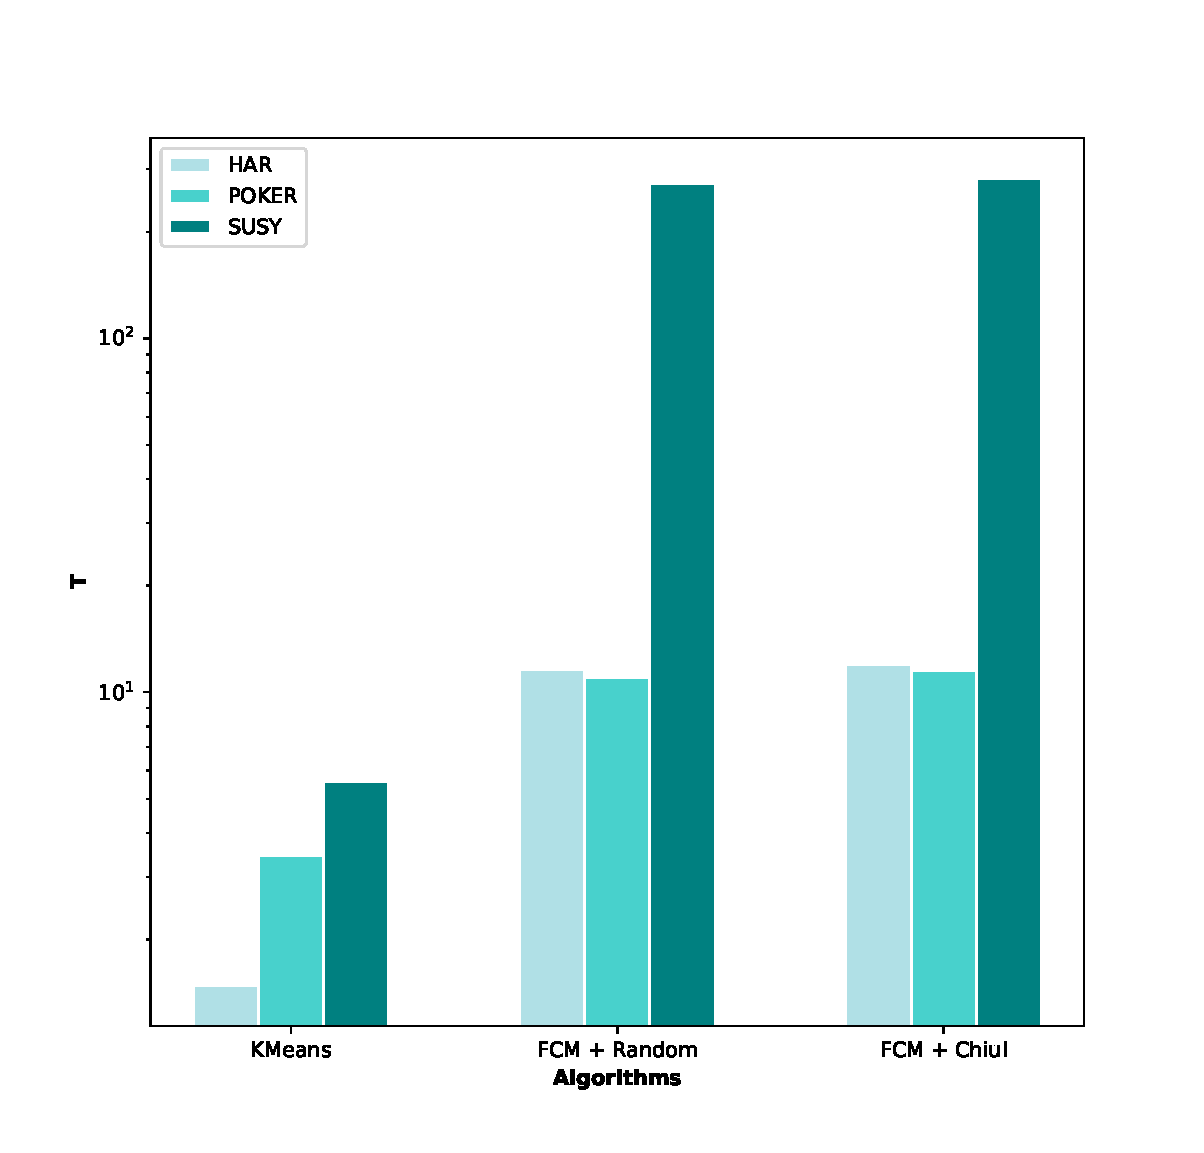
\includegraphics[width=.7\textwidth]{bar-chart.pdf}
\caption{Comparison of execution time of the three clustering algorithms on the three data sets employed, using 250 centroids. The vertical axis represents the time in minutes, and is measured on a logarithmic scale.}
\label{fig:bar-chart}
\end{figure}

\subsection{Regression algorithms}

Having reviewed all the classification algorithms implemented, we move on to the regression tasks. In this regard we will be experimenting with the adapted version of the subtractive clustering algorithm to build a FRBS, and also with the algorithm developed by Wang and Mendel for accomplishing that same goal. In both cases we build a Mamdani type fuzzy inference system. First of all we constructed a toy example to visualize how these algorithms performed on a simple function estimation, and also to ensure that they worked as intended. The result is shown on Figure \ref{fig:sin}.

\begin{figure}[h!]
\centering
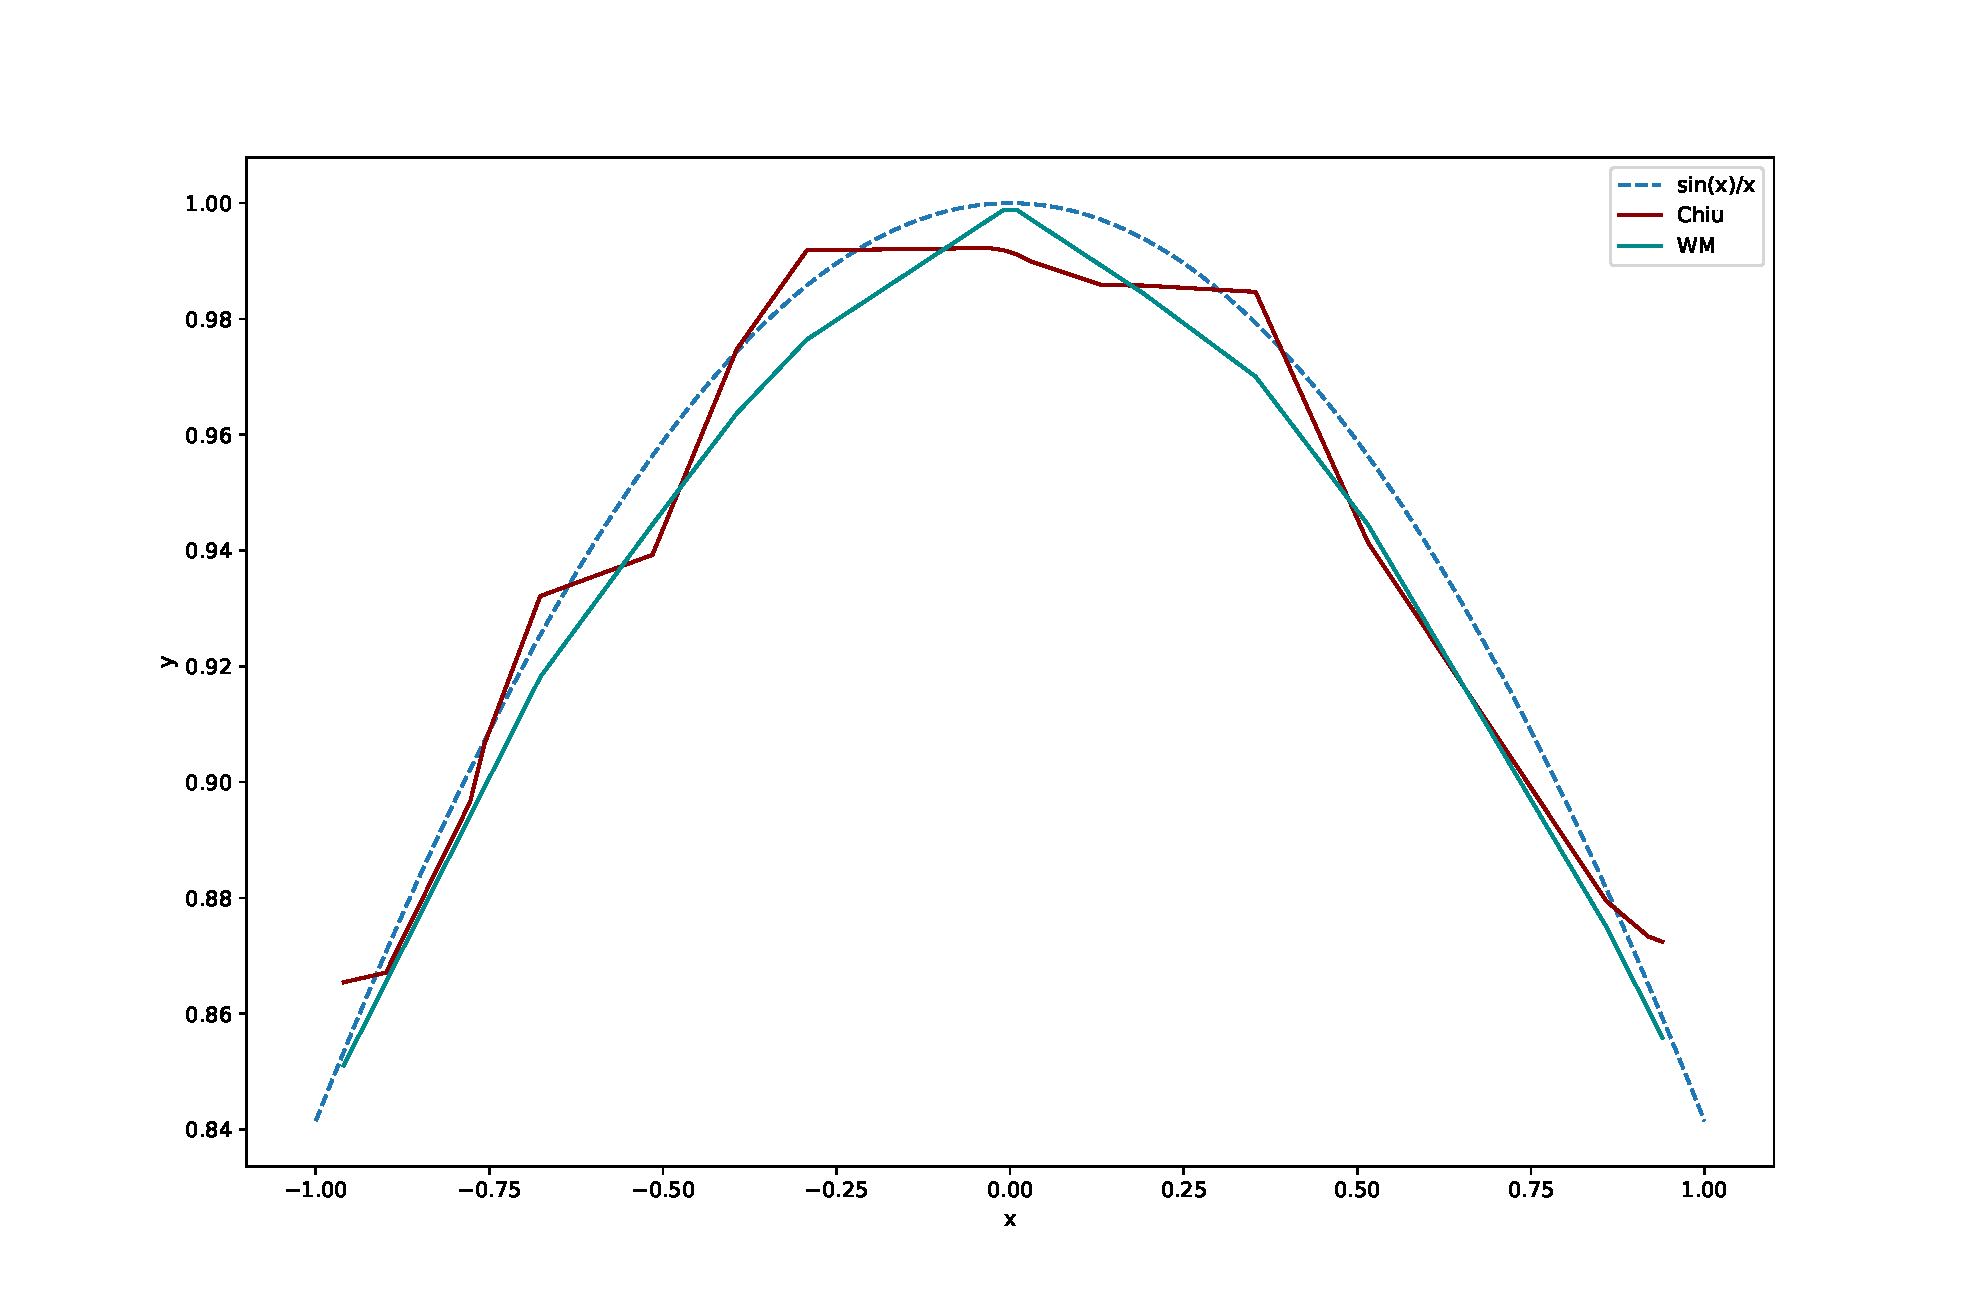
\includegraphics[width=.7\textwidth, height=9cm]{sin}
\caption{Model obtained with the Wang \& Mendel and the subtractive clustering algorithms when trying to estimate the function $\sin(x)/x$ from a few points on its domain.}
\label{fig:sin}
\end{figure}

Now we focus on the real experimentation on our two regression data sets. As we did with the classification models, we have included some well-known algorithms for comparison: a Random Forest regressor and a standar linear regressor with L2 regularization. Apart from the execution time, which is our main concern, the metric to analyze in this case is the MSE. In the case of the Wang \& Mendel algorithm we use the same number of partitions across every dimension, and in the case of the subtractive clustering algorithm we fix the stopping conditions in the same way as we before.

We begin with the smaller QAW data set, whose execution results can be seen in Table \ref{tab:qaw}. We can see that the standard linear regression is the winner in this case getting the best result in a negligible amount of time. On the other hand, what may seem strange is that the Random Forest regressor did not outperform almost any other algorithm, probably due to overfitting. Of the three different configurations tried for the Wang \& Mendel algorithm, we observe that the best one is the one with less partitions (a total of 7), and it seems that increasing the number of partitions up to 15 results in a higher prediction error while also increasing the execution time. Lastly, Chiu's algorithm does quite well in this case, reaching the second best overall score in a reasonable amount of time. In this case the algorithm profits from a smaller neighbourhood radius, and the more cluster centers selected, the better the results.

\begin{table}[h!]
\centering
\caption{Experimental results of every regression algorithm considered for the QAW data set.}
\label{tab:qaw}
\begin{tabular}{ccccc}
\toprule
\multicolumn{2}{c}{Algorithm} & Centroids & MSE & T\\ \midrule
  Random Forest & & -- & 0.779 & 0.22 \\
  Ridge Regression & & -- & \textbf{0.098} &0.08\\
 \multirow{3}{*}{Wang \& Mendel} & $N=3$ & -- & 0.655 & 0.06\\
  & $N=5$ & -- & 1.374 & 0.14\\
  & $N=7$ & -- & 2.195 & 0.30\\
 \multirow{3}{*}{ChiuI} & $r_a=0.5$ &  2845 & 0.382 & 2.11\\
  & $r_a=0.75$ &  492 & 0.664 & 0.51\\
  & $r_a=1.0$ &  225 & 0.827 & 0.31\\ \bottomrule
\end{tabular}
\end{table}

Similarly, the results of the executions on the GSA data set are summarized in Table \ref{tab:gsa}. The comparison algorithms behave in a similar way as in the previous case, but now the Random Forest does perform fairly well. However, in the Wang \& Mendel algorithm we observe an effect opposed to what we saw before, because in this case it seems that a higher number of partitions is better. This diametral change in the situation should not come as a surprise, since now we are considering 4 million points more, and it makes sense that a few more rules are needed to better explain the behaviour of the system.

The behaviour exhibited by Chiu's algorithm is also in direct opposition to the previous case, because now the results are better (and of course faster) with a lower number of clusters. This can be explained because, in a Big Data setting, having a huge quantity of points could mean that clusters can take up more space, and fewer of them are needed to accurately describe the idiosyncrasies of the data. With regard to the execution time, the Wang \& Mendel algorithm with 15 partitions finishes in less than half the time as the subtractive clustering algorithm, and also produces a better result. However, in both cases we can say that the time taken to finish is relatively low, especially when compared with the classification algorithms for the similarly sized SUSY data set.

\begin{table}[h!]
\centering
\caption{Experimental results of every regression algorithm considered for the GSA data set.}
\label{tab:gsa}
\begin{tabular}{ccccc}
\toprule
\multicolumn{2}{c}{Algorithm} & Centroids & MSE & T\\ \midrule
  Random Forest & & -- & \textbf{0.301} & 3.59 \\
  Ridge Regression & & -- & 0.392 &0.25\\
 \multirow{3}{*}{Wang \& Mendel} & $N=3$ & -- & 0.539 & 0.55\\
  & $N=5$ & -- & 0.592 & 1.63\\
  & $N=7$ & -- & 0.395 & 3.13\\
 \multirow{3}{*}{ChiuI} & $r_a=0.3$ & 438 & 0.627 & 8.89\\
  & $r_a=1.0$ &  246 & 0.471 & 8.13\\
  & $r_a=1.5$ &  225 & 0.453 & 8.72\\ \bottomrule
\end{tabular}
\end{table}

Finally, we show a comparison of the execution time of all the algorithms in both data sets. In this case the conclusions drawn are even better, since it can be seen in Figure \ref{fig:bar-chart-2} that the execution times remain in the same order of magnitude in each data set, but they also do not differ a lot when visualized together.

\begin{figure}[h!]
\centering
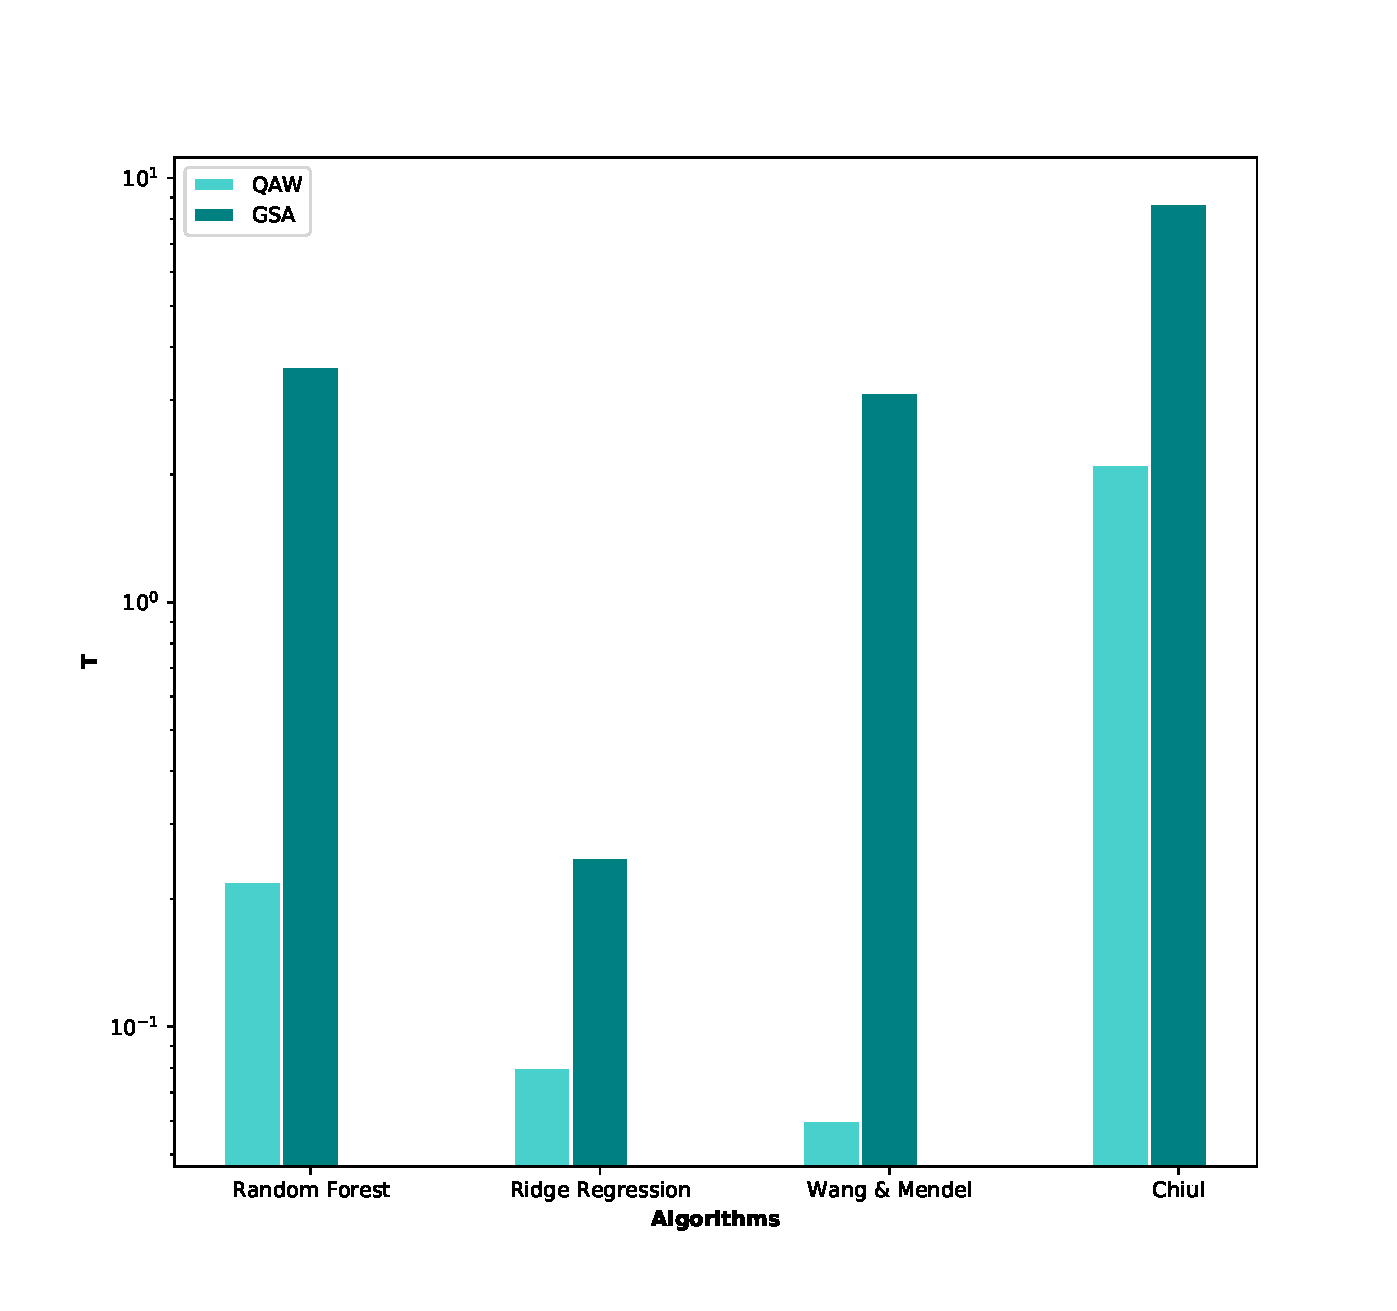
\includegraphics[width=.7\textwidth]{bar-chart-2.pdf}
\caption{Comparison of execution time of the four regression algorithms on the two data sets employed. The vertical axis represents the time in minutes, and is measured on a logarithmic scale.}
\label{fig:bar-chart-2}
\end{figure}
